% vim: set tw=78 aw sw=2 sts=2 noet:

\section{Hand gesture recognition}

\begin{frame}{Rock-Paper-Scissors}
  \begin{figure}
	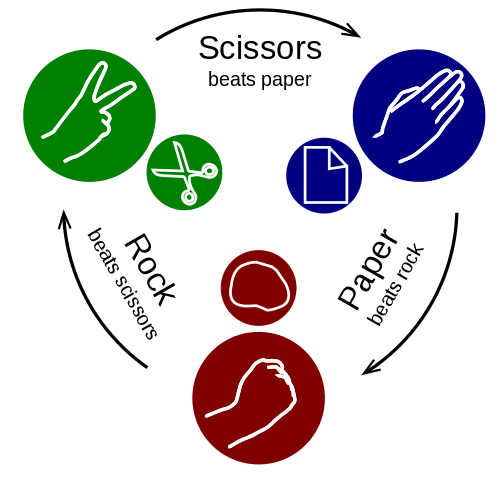
\includegraphics[width=\linewidth,height=0.75\textheight,keepaspectratio]{images/502px-Rock-paper-scissors.svg.png}
	\caption{wikipedia.org}
  \end{figure}
\end{frame}

\begin{frame}{Data}
  \begin{itemize}
	\item Google MediaPipe's Rock-Paper-Scissors dataset for hand gesture
	recognition
	  \begin{itemize}
		\item Has a "none" class
		\item Contains 125 images for each class
		\item Images have various sizes
		\item Images have 3 color channels per pixel (RGB)
	  \end{itemize}
	\item Laurence Moroney's Rock-Paper-Scissors dataset (published by Sani
	Kamal on Kaggle)
	  \begin{itemize}
		\item Contains 964 images for each class split into training set (840) and testing set (124)
		\item Images are 300x300 pixels
		\item Images have 3 color channels per pixel (RGB)
	  \end{itemize}
  \end{itemize}
\end{frame}

\begin{frame}{Train a CNN model - Prerequisites}
  \begin{itemize}
	\item To be run on host
	\item Python
	\item TensorFlow Lite
	\item OpenCV
  \end{itemize}
\end{frame}

\begin{frame}{Train a CNN model - Algorithm}
  \begin{enumerate}
	\item Build the model
	\item Configure the model
	\item Load the data
	\item Train the model
	\item Convert to lite model
  \end{enumerate}
\end{frame}

\begin{frame}[fragile]{Train a CNN model - 1. Build the model}
  \lstset{basicstyle=\ttfamily\small, numbers=left, columns=fullflexible}
  \begin{lstlisting}
base_model = tf.keras.applications.ResNet50(
  include_top = False,
  input_shape = (96, 96, 3),
  pooling = "avg"
)

base_model.trainable = False

model = tf.keras.models.Sequential()

model.add(base_model)
model.add(tf.keras.layers.Dropout(rate = 0.5))
model.add(
  tf.keras.layers.Dense(
    units = 3,
    activation = tf.keras.activations.softmax
  )
)
  \end{lstlisting}
\end{frame}

\begin{frame}[fragile]{Train a CNN model - 2. Configure the model}
  \lstset{basicstyle=\ttfamily\small, numbers=left, columns=fullflexible}
  \begin{lstlisting}
model.compile(
  optimizer = tf.keras.optimizers.SGD(),
  loss = "categorical_crossentropy",
  metrics = ["accuracy"]
)
  \end{lstlisting}
\end{frame}

\begin{frame}[fragile]{Train a CNN model - 3. Load the data}
  \lstset{basicstyle=\ttfamily\small, numbers=left, columns=fullflexible}
  \begin{lstlisting}
LABELS = ["rock", "paper", "scissors"]

training_data = tf.keras.utils.image_dataset_from_directory(
  "data/training",
  image_size = (96, 96),
  label_mode = "categorical",
  class_names = LABELS
)

validation_data = tf.keras.utils.image_dataset_from_directory(
  "data/validation",
  image_size = (96, 96),
  label_mode = "categorical",
  class_names = LABELS
)
  \end{lstlisting}
\end{frame}

\begin{frame}[fragile]{Train a CNN model - 4. Train the model}
  \lstset{basicstyle=\ttfamily\small, numbers=left, columns=fullflexible}
  \begin{lstlisting}
model.fit(
  training_data,
  epochs = 10,
  validation_data = validation_data
)
  \end{lstlisting}
\end{frame}

\begin{frame}[fragile]{Train a CNN model - 5. Convert to lite model}
  \lstset{basicstyle=\ttfamily\small, numbers=left, columns=fullflexible}
  \begin{lstlisting}
converter = tf.lite.TFLiteConverter.from_keras_model(model)
converter.optimizations = [tf.lite.Optimize.DEFAULT]

lite_model = converter.convert()
  \end{lstlisting}
\end{frame}

\begin{frame}[fragile]{Train on small dataset}
  \begin{itemize}
	\item Random shuffle and split the images into:
	\begin{itemize}
	  \item 80\% for training (300 images)
	  \item 20\% for validation (75 images)
	\end{itemize}
  \end{itemize}
  \lstset{basicstyle=\tiny, numbers=left}
  \begin{lstlisting}
Epoch 1/10
9s - loss: 2.0545 - accuracy: 0.5700 - val_loss: 3.0788 - val_accuracy: 0.4800
Epoch 2/10
5s - loss: 1.4671 - accuracy: 0.7300 - val_loss: 1.5156 - val_accuracy: 0.7467
Epoch 3/10
5s - loss: 0.6304 - accuracy: 0.8567 - val_loss: 0.1994 - val_accuracy: 0.9467
Epoch 4/10
5s - loss: 0.3750 - accuracy: 0.9100 - val_loss: 0.3066 - val_accuracy: 0.9067
Epoch 5/10
5s - loss: 0.4212 - accuracy: 0.8933 - val_loss: 0.2647 - val_accuracy: 0.9333
Epoch 6/10
5s - loss: 0.3357 - accuracy: 0.8933 - val_loss: 0.1780 - val_accuracy: 0.9200
Epoch 7/10
5s - loss: 0.1435 - accuracy: 0.9533 - val_loss: 0.1747 - val_accuracy: 0.9733
Epoch 8/10
5s - loss: 0.2573 - accuracy: 0.9267 - val_loss: 0.1982 - val_accuracy: 0.9333
Epoch 9/10
5s - loss: 0.1846 - accuracy: 0.9367 - val_loss: 0.1352 - val_accuracy: 0.9867
Epoch 10/10
5s - loss: 0.1590 - accuracy: 0.9433 - val_loss: 0.1135 - val_accuracy: 0.9600
  \end{lstlisting}
  \begin{itemize}
	\item Duration: 2m15s
	\item Model size: 23MB
  \end{itemize}
\end{frame}

\begin{frame}{Test on small dataset}
Using the testing dataset of the big dataset (124 images per class)
  \begin{table}
	\begin{tabular}{|c|c|c|}
	  \hline
		\textbf{Gesture} & \textbf{Correct predictions} & \textbf{Accuracy (\%)} \\
	  \hline
		Rock & 108 & 87.09 \\
	  \hline
		Paper & 124 & 100 \\
	  \hline
		Scissors & 8 & 6.45 \\
	  \hline
	  \hline
		All & 240 out of 372 & 64.51 \\
	  \hline
	\end{tabular}
  \end{table}
\end{frame}

\begin{frame}[fragile]{Train on big dataset}
  \begin{itemize}
	\item Random shuffle and split the training set:
	\begin{itemize}
	  \item 80\% for training (2016 images)
	  \item 20\% for validation (504 images)
	\end{itemize}
  \end{itemize}
  \lstset{basicstyle=\tiny, numbers=left}
  \begin{lstlisting}
Epoch 1/10
37s - loss: 1.0362 - accuracy: 0.8284 - val_loss: 0.1478 - val_accuracy: 0.9385
Epoch 2/10
35s - loss: 0.1554 - accuracy: 0.9444 - val_loss: 0.0386 - val_accuracy: 0.9861
Epoch 3/10
35s - loss: 0.1092 - accuracy: 0.9608 - val_loss: 0.0256 - val_accuracy: 0.9901
Epoch 4/10
35s - loss: 0.0918 - accuracy: 0.9668 - val_loss: 0.0133 - val_accuracy: 0.9980
Epoch 5/10
35s - loss: 0.0589 - accuracy: 0.9797 - val_loss: 0.0325 - val_accuracy: 0.9861
Epoch 6/10
35s - loss: 0.0500 - accuracy: 0.9826 - val_loss: 0.0091 - val_accuracy: 0.9980
Epoch 7/10
35s - loss: 0.0361 - accuracy: 0.9896 - val_loss: 0.0070 - val_accuracy: 1.0000
Epoch 8/10
35s - loss: 0.0410 - accuracy: 0.9856 - val_loss: 0.0071 - val_accuracy: 1.0000
Epoch 9/10
35s - loss: 0.0310 - accuracy: 0.9886 - val_loss: 0.0074 - val_accuracy: 1.0000
Epoch 10/10
35s - loss: 0.0395 - accuracy: 0.9866 - val_loss: 0.0046 - val_accuracy: 1.0000
  \end{lstlisting}
  \begin{itemize}
	\item Duration: 7m10s
	\item Model size: 23MB
  \end{itemize}
\end{frame}

\begin{frame}{Test on big dataset}
Using its own testing dataset (124 images per class)
  \begin{table}
	\begin{tabular}{|c|c|c|}
	  \hline
		\textbf{Gesture} & \textbf{Correct predictions} & \textbf{Accuracy (\%)} \\
	  \hline
		Rock & 124 & 100 \\
	  \hline
		Paper & 122 & 98.38 \\
	  \hline
		Scissors & 97 & 78.22 \\
	  \hline
	  \hline
		All & 343 out of 372 & 92.20 \\
	  \hline
	\end{tabular}
  \end{table}
\end{frame}

\begin{frame}{Inference using the trained CNN model}
  \begin{itemize}
	\item Same hardware setup
	\item Same software dependencies
	\item Same C++ code
  \end{itemize}
\end{frame}

\begin{frame}{Demo}
  \begin{figure}
	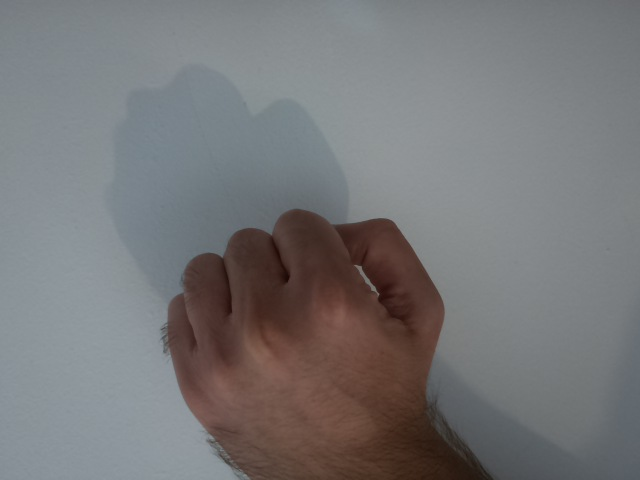
\includegraphics[width=0.33\linewidth,height=0.5\textheight,keepaspectratio]{../images/rock_input.jpeg}%
	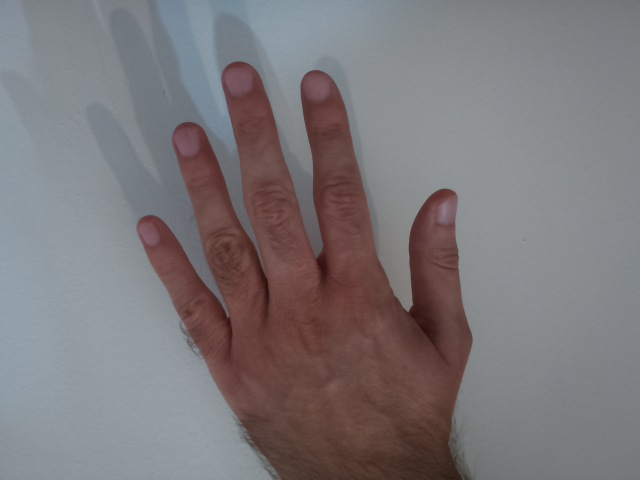
\includegraphics[width=0.33\linewidth,height=0.5\textheight,keepaspectratio]{../images/paper_input.jpeg}%
	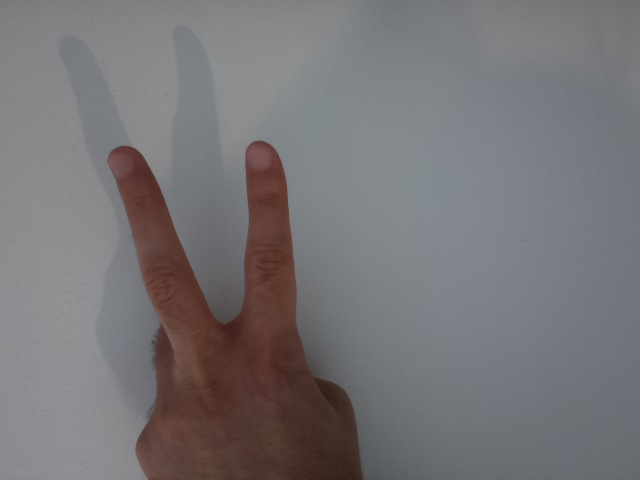
\includegraphics[width=0.33\linewidth,height=0.5\textheight,keepaspectratio]{../images/scissors_input.jpeg}
  \end{figure}
\end{frame}

\begin{frame}{Demo - Small dataset results}
  \begin{figure}
	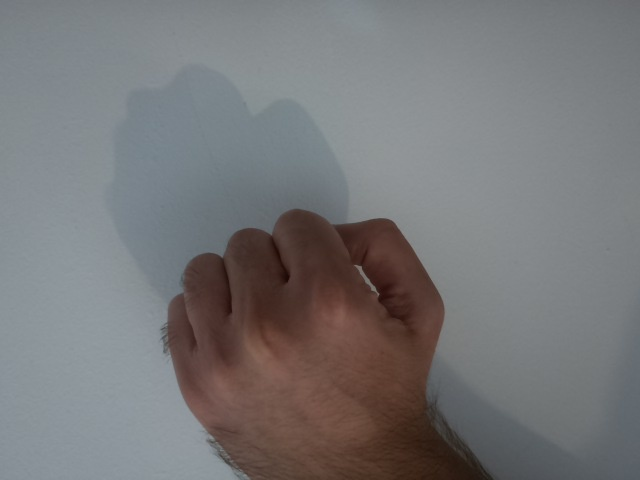
\includegraphics[width=0.33\linewidth,height=0.5\textheight,keepaspectratio]{images/rock_small_dataset_output.jpeg}%
	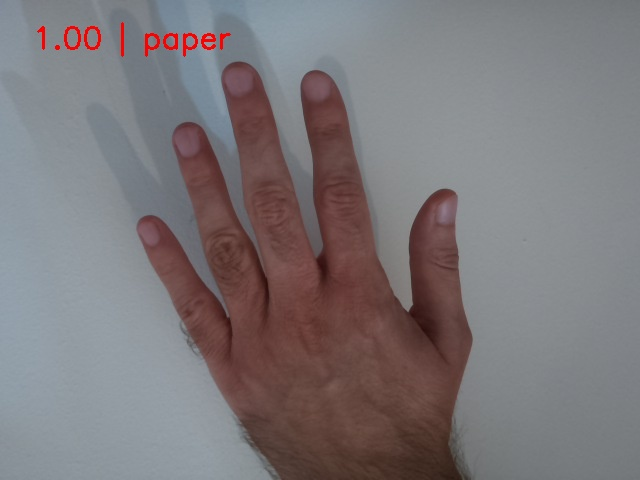
\includegraphics[width=0.33\linewidth,height=0.5\textheight,keepaspectratio]{images/paper_small_dataset_output.jpeg}%
	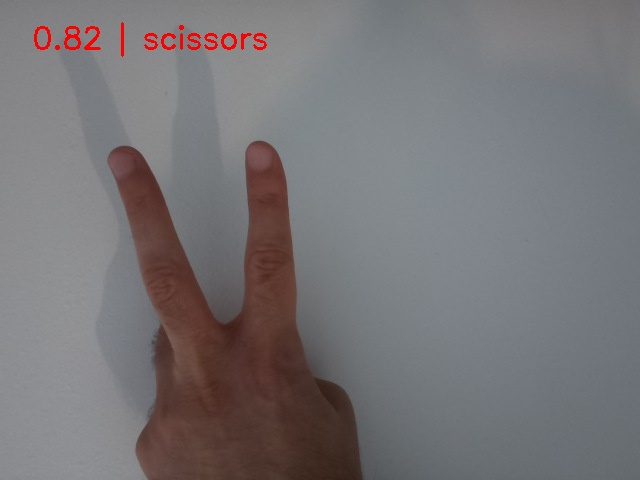
\includegraphics[width=0.33\linewidth,height=0.5\textheight,keepaspectratio]{images/scissors_small_dataset_output.jpeg}
  \end{figure}
  \ttfamily 0.54 | scissors \\
  \ttfamily 0.31 | paper \\
  \ttfamily 0.15 | rock \\
  \ttfamily ambiguous results
\end{frame}

\begin{frame}{Demo - Big dataset results}
  \begin{figure}
	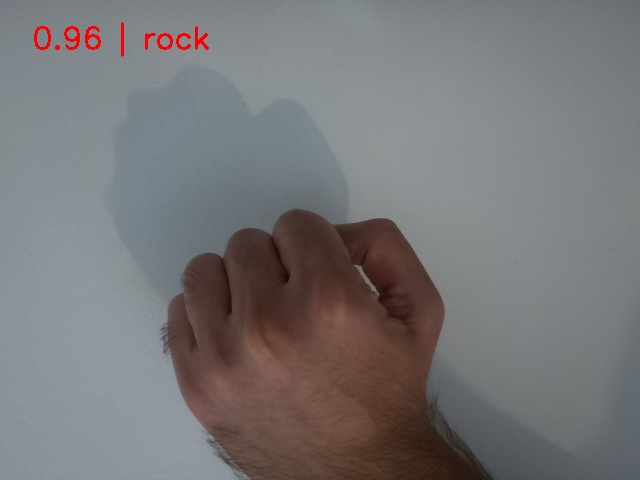
\includegraphics[width=0.33\linewidth,height=0.5\textheight,keepaspectratio]{images/rock_output.jpeg}%
	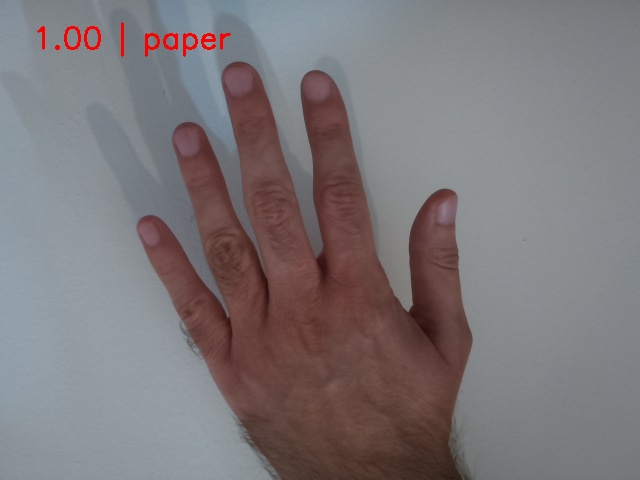
\includegraphics[width=0.33\linewidth,height=0.5\textheight,keepaspectratio]{images/paper_output.jpeg}%
	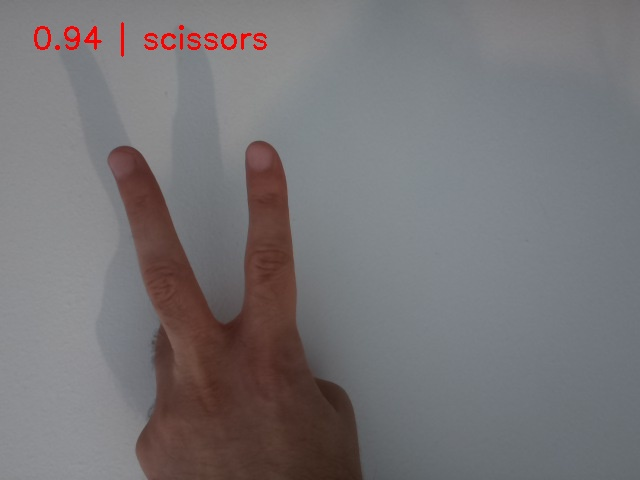
\includegraphics[width=0.33\linewidth,height=0.5\textheight,keepaspectratio]{images/scissors_output.jpeg}
  \end{figure}
\end{frame}

\begin{frame}{Performance}
  \begin{itemize}
	\item Compilation duration: 35s
	\item Running duration: 1s
  \end{itemize}
  \begin{table}
    {\tiny
	\begin{tabular}{|c|c|}
	  \hline
		\textbf{Number of threads} & \textbf{Inference duration (ms)} \\
	  \hline
		1 & 151 \\
	  \hline
		2 & 98 \\
	  \hline
		3 & 80 \\
	  \hline
		4 & 71 \\
	  \hline
		5 & 189 \\
	  \hline
	\end{tabular}
	}
  \end{table}
  \begin{figure}
	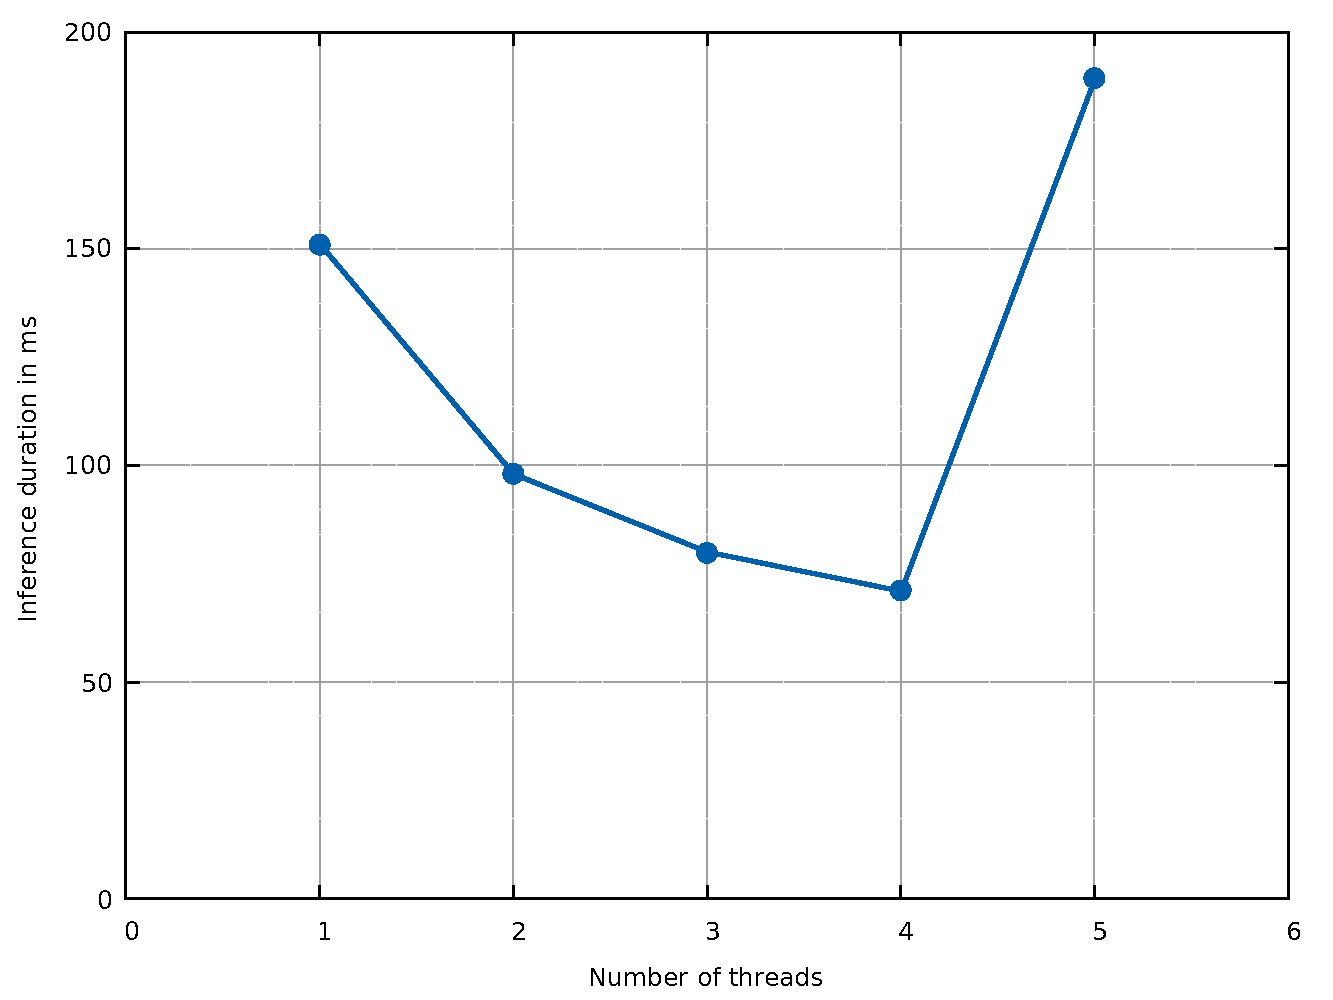
\includegraphics[width=\linewidth,height=0.5\textheight,keepaspectratio]{images/inference_duration_rps.pdf}
  \end{figure}
  \begin{itemize}
	\item Memory consumption with 4 threads: 118MB
  \end{itemize}

\end{frame}

\begin{frame}{Live camera stream}
  \begin{itemize}
	\item libcamera backend
	\item gstreamer middleware
	\item OpenCV frontend
  \end{itemize}
\end{frame}

\begin{frame}[fragile]{Live camera stream}
  \lstset{basicstyle=\ttfamily\small, showstringspaces=false, numbers=left,
  columns=fullflexible}
  \begin{lstlisting}
static constexpr const char *GstreamerPipeline{R"(
    libcamerasrc !
    video/x-raw,
    width=(int)640,
    height=(int)480,
    framerate=(fraction)10/1 !
    videoconvert !
    appsink
)"};

cv::VideoCapture camera{
  GstreamerPipeline,
  cv::CAP_GSTREAMER
};

cv::Mat image;
camera >> image;
  \end{lstlisting}
\end{frame}

\begin{frame}{Live inference - Algorithm}
  \begin{enumerate}
	\item Create image classifier
	\item Open camera
	\item Do in a loop:
	\begin{enumerate}
	  \item Read image from camera
	  \item Use classifier to run inference on image
	  \item Show predictions
	\end{enumerate}
  \end{enumerate}
\end{frame}

\begin{frame}{Live inference - Demo}
\end{frame}

\begin{frame}{Live inference - Performance}
Stats for 4 threads:
  \begin{itemize}
	\item Inference duration: 71ms
	\item Loop duration: 96ms
	\item Memory consumption: 123MB
  \end{itemize}
\end{frame}

\begin{frame}{Rock-Paper-Scissors game mode}
On each round the AI:
  \begin{enumerate}
	\item Chooses Rock, Paper or Scissors uniformly at random
	\item Infers the human's hand gesture
	\item Computes the outcome
  \end{enumerate}
\end{frame}

\begin{frame}{Rock-Paper-Scissors game mode - Demo}
  \begin{figure}
	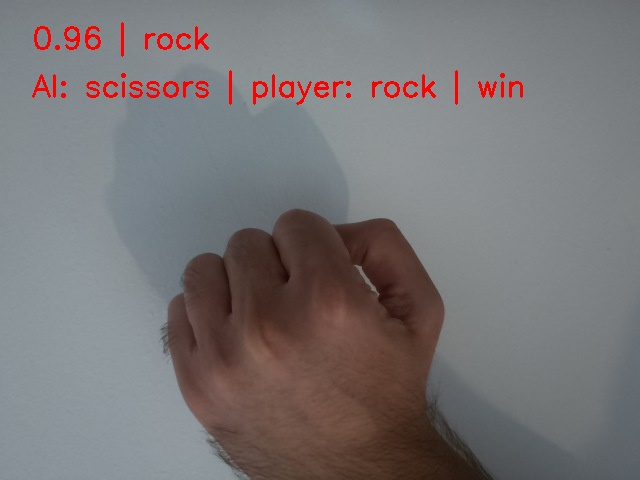
\includegraphics[width=0.33\linewidth,height=0.5\textheight,keepaspectratio]{images/rock_game_win.jpeg}%
	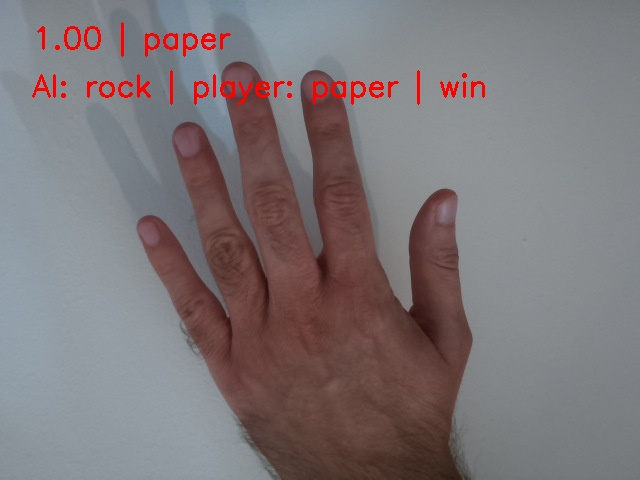
\includegraphics[width=0.33\linewidth,height=0.5\textheight,keepaspectratio]{images/paper_game_win.jpeg}%
	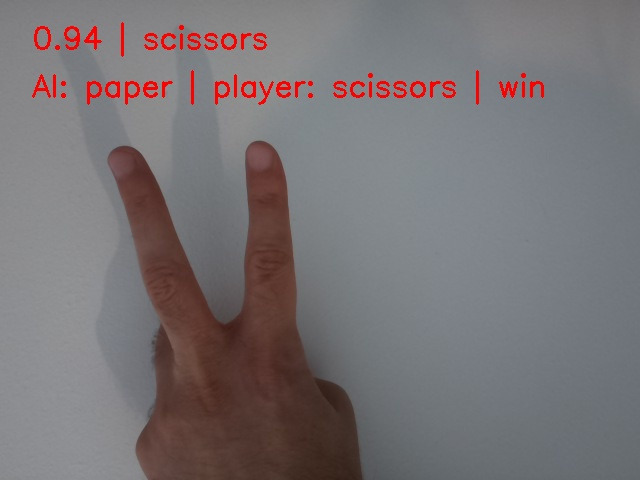
\includegraphics[width=0.33\linewidth,height=0.5\textheight,keepaspectratio]{images/scissors_game_win.jpeg}
	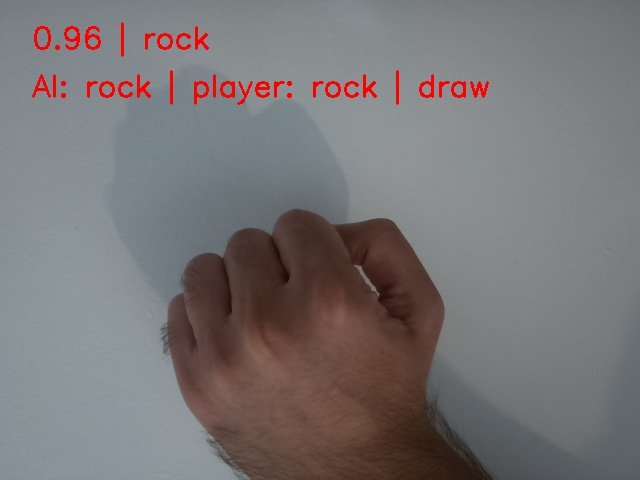
\includegraphics[width=0.33\linewidth,height=0.5\textheight,keepaspectratio]{images/rock_game_draw.jpeg}%
	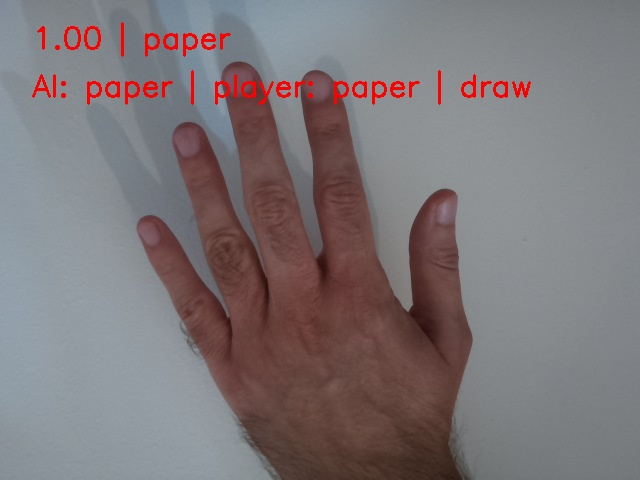
\includegraphics[width=0.33\linewidth,height=0.5\textheight,keepaspectratio]{images/paper_game_draw.jpeg}%
	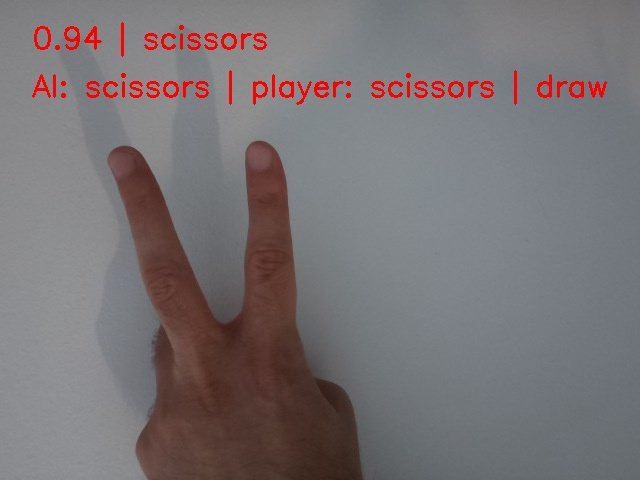
\includegraphics[width=0.33\linewidth,height=0.5\textheight,keepaspectratio]{images/scissors_game_draw.jpeg}
	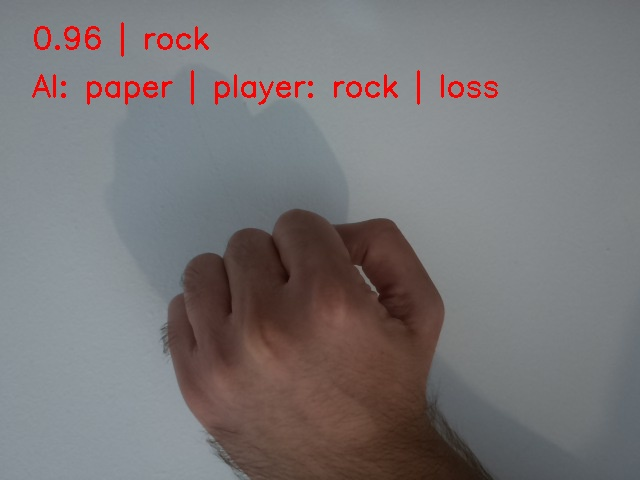
\includegraphics[width=0.33\linewidth,height=0.5\textheight,keepaspectratio]{images/rock_game_loss.jpeg}%
	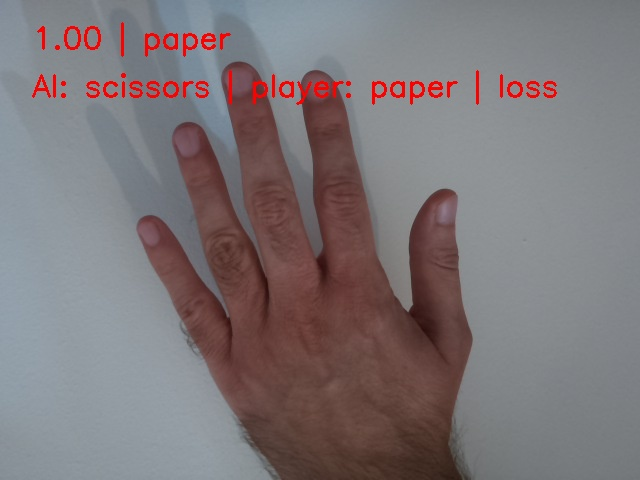
\includegraphics[width=0.33\linewidth,height=0.5\textheight,keepaspectratio]{images/paper_game_loss.jpeg}%
	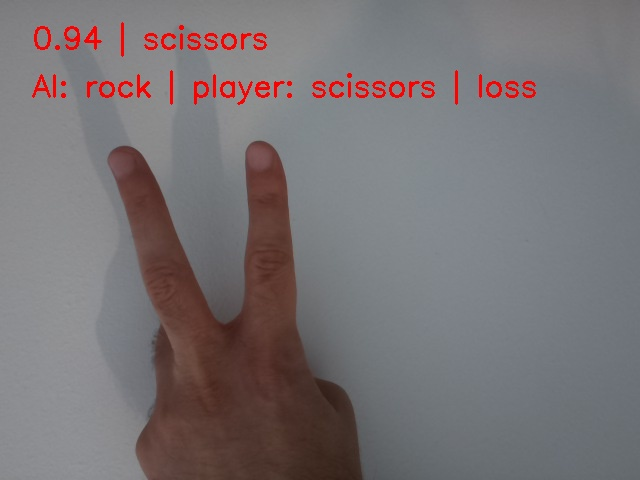
\includegraphics[width=0.33\linewidth,height=0.5\textheight,keepaspectratio]{images/scissors_game_loss.jpeg}
  \end{figure}
\end{frame}

